\documentclass[a4paper, 11pt]{article}
\usepackage{comment} % enables the use of multi-line comments (\ifx \fi) 
\usepackage{lipsum} %This package just generates Lorem Ipsum filler text.
\usepackage{a4wide}
\usepackage{url}
\usepackage[utf8]{inputenc}
\usepackage{fancyhdr}
\usepackage{graphicx}

\lhead{\textbf{Paper Ashes}: Art + Story Bible \\ A \textbf{realtime grand strategy game} for \textit{PC/Mac}}
\rhead{v.0.0.1 \today \\ Page \thepage}
\cfoot{}

\DeclareGraphicsExtensions{.pdf,.png,.jpg,.jpeg}

\renewcommand{\headrulewidth}{0.4pt}
\renewcommand{\footrulewidth}{0.4pt}

\widowpenalties 1 10000
\raggedbottom

\begin{document}
\pagestyle{fancy}
\setlength\parindent{0pt}
\setlength{\parskip}{1em}
\renewcommand{\baselinestretch}{1.5}

\section*{Artwork and Key Concepts}

The horror of war and the historical account of it (in the sense of compilation and academia). A filtered and sanitized treatement of all the blood and suffering.

All the visuals should be inspired by art from the early XX century, especially coloured sketches and press comics (see below austrian military sketch) and also mixing in elements of comics of the era (imagine Tintin with a serious, grave and dire approach). For the music and sounds we'll go with orchestrated classical, nothing too vangardist, modernism is ok. Don't include anything that's subjective (i.e. impressionism), we have to show the horrors of war are objective but the art style shouldn't be too realistic either: i.e. coloured but toned down 3D models and 2D graphics and menus.

For artwork details a good start is \url{https://en.wikipedia.org/wiki/Austro-Hungarian_Army} and for menus and UI \url{http://digitale-bibliothek.belvedere.at/viewer/browse/hagenbund/-/1/-/-/}.

\begin{figure}[h]
    \centering
	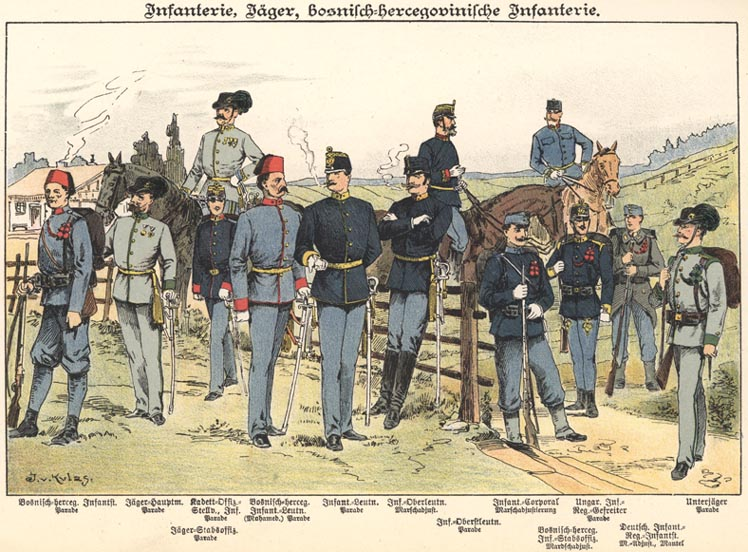
\includegraphics[keepaspectratio=true,width=\textwidth,height=300px]{austrian_infantry}
\end{figure}

\section*{Setting}

You're a mid-level officer of the Republic of Mogyana, a fictional long-standing Republic on a fictional modern world with technology at the level of early XX century real world and a culture roughly based off old Austria-Hungary, also not culturally-united at all.


Said Republic military hierarchy was recently destroyed by plague, famine and a civil war caused as a reaction to these. Nobility still exists in Mogyanan society after a peaceful transition from a monarchy to a republic, although it's only referred to the fact they're landowners and titles don't grant any special powers over Mogyanan citizens. Noblemen usually end up elected as governors and ministers, given their financial power to define and modify the living conditions of the commoners. Military have nobility titles without ownership of land, mostly as a cerimonial thing (but could legitimize an aspiring governor trying to take and seize power).

With the troops you command and the territory under your control you decide to step up and declare independence to make a stable state that can guard the people against other armies and general turmoil. You have to make decisions about government system, laws, army power within the state and most importantly to wage war and `free` other states and organisations putting them under your control. 

You decide how to go, but the game will make, implicitely, the consequences of your decisions painfully obvious: the reasons Mogyana fell into disarray were dumb decisions made by people, and your rule will be no different. Will your rule endure internal and external strife long enough? Would you be able to subjugate all of the old enemies of the Republic? Will your rule make the lifes of the commoners better or worse? Will it be at the cost of your personal power? These are all the questions that gameplay will have to answer.

\section*{Characters}

\subsubsection*{You}
A nondescript soldier of the Mogyana army, you are young, served a few years then got promoted to leader of a bunch of rookies due to the power vacuum created by the crisis. As such you and your soldiers are not experienced, not well trained and not loyal, problems you'll have to deal with. We deliberately exclude the faction you are part of, but canonically the main character should be a Republican (see below). Gender and race explicitely nondescript.

As of now we didn't design relevant characters you'll interact with. The inclusion of personal interaction would enrich the experience or dilute it?

\section*{Factions}

We include here factions you can join, make alliances or wage war on.

\subsubsection*{Mogyanan Republicans}

The loyal side of the civil war. They believe the government that irresponsibly let his citizens starve and die en masse without providing any aid to their subjects will be able to revive the country. Formed mostly by Mogyanan noblemen that were democratically appointed to gobern over provinces, which gave them the ability to sell favors to the voters to perpetuate themselves in power.

\subsubsection*{Mogyanan Monarchists}

The rebelling side of the civil war. Mostly composed of disgruntled peasants and burghers and low nobility that were the most damaged classes from the Mogyanan crisis. They believe that reinstating the heir of the expelled monarchy is the way to go to restore social order, which implies democracy is the root of all problems in the country. Most of them also expect to curry favor from the reinstated monarch.

\subsubsection*{Northern Empire}

The remnants of a great empire of old (based off the Holy Roman Empire) that believe Mogyana should be a subject of the empire like in the gold olden days. They believe they should reunite the Empire and rule over all of the imperial subjects, being the continuator of true Imperial lineage. They are not in active war against the Southern Empire, but the political climate is not peaceful either.

\subsubsection*{Southern Empire}

The remnants of a great empire of old that also believe Mogyana should be a subject of the empire like in the gold olden days, these are a democratic constitutional monarchy based off mediterranean nations, a gradual transition from Imperial values due to being the poorest region of the former united Empire, that subsequently caused crises and disgruntled nobility and burghers that progressively demanded more power from the ruling monarch. The Southern Empire splitted from the Northern half a millenia ago, during an imperial succesion crisis and the following civil war waged by opposing noblemen.

\subsubsection*{The Ayyubid Dynasty}

A confederation of tribes from the far east (based off the Ottoman Empire), ruled by an emperor. The emperor has to continuously curry favor from the rulers of the minor clans or risk rebellion, so it's actually a democratic government in a weird way. It differs culturally and on religious issues with all the other nations in the game, and believes conquering and assimilating them is a task given to them by god.

\end{document}
